\documentclass[12pt]{article}
\usepackage[top=1in, bottom=1in, left=.75in, right=.75in]{geometry}

\usepackage{amsmath}
\usepackage{fancyhdr}
\usepackage{graphicx}
\usepackage{txfonts}
\usepackage{multicol,pgfplots}
\usepackage{wrapfig}
\usepackage[scaled=0.86]{helvet}
\renewcommand{\emph}[1]{\textsf{\textbf{#1}}}
\usepackage{anyfontsize}
% \usepackage{times}
% \usepackage[lf]{MinionPro}

%%TIKZ
\usepackage{tikz,pgfplots}
\usetikzlibrary{calc}
\usetikzlibrary{shapes}
%\pgfplotsset{my style/.append style={axis x line=middle, axis y line=middle, xlabel={$x$}, ylabel={$y$}, axis equal }}
%OTHER
%\pgfplotsset{my style/.append style={axis x line=middle, axis y line=middle, xlabel={}, ylabel={}}}

\pgfplotsset{my style/.append style={axis x line=middle, axis y line=middle, 
xlabel=$x$,ylabel=$y$,
every axis x label/.style={
    at={(ticklabel* cs:1)},
    anchor=west,
},
every axis y label/.style={
    at={(ticklabel* cs:1)},
    anchor=south,
},}}

\def\degC{{}^\circ{\rm C}}
\def\ra{\rightarrow}

\newcommand*\circled[1]{\tikz[baseline=(char.base)]{
            \node[shape=ellipse,draw,inner sep=2pt] (char) {#1};}}

\newcommand{\blank}[1]{\rule{#1}{0.75pt}}

\parindent 0pt
\parskip 4pt
\pagestyle{fancy}
\fancyfoot[C]{\emph{\thepage}}
\fancyhead[L]{\ifnum \value{page} > 1\relax\emph{Math 251: Final Exam}\fi}
\fancyhead[R]{\ifnum \value{page} > 1\relax\emph{28 April 2020}\fi}
\headheight 15pt
\renewcommand{\headrulewidth}{0pt}
\renewcommand{\footrulewidth}{0pt}
\let\ds\displaystyle
\def\continued{{\emph {Continued....}}}
\def\continuing{{\emph {Problem \arabic{probcount} continued....}}\par\vskip 4pt}

\newcounter{probcount}
\newcounter{subprobcount}
\newcommand{\thesubproblem}{\emph{\alph{subprobcount}.}}

\def\problem#1{\setcounter{subprobcount}{0}%
\addtocounter{probcount}{1}{\emph{\arabic{probcount}.\hskip 1em(#1)}}\par}

\def\ecproblem#1{{\emph{Extra Credit. \hskip 1em(#1)}}\par}

\def\subproblem#1{\par\hangindent=1em\hangafter=0{%
\addtocounter{subprobcount}{1}\thesubproblem\emph{#1}\hskip 1em}}

\def\probskip{\vskip 10pt}
\def\medprobskip{\vskip 2in}
\def\subprobskip{\vskip 45pt}
\def\bigprobskip{\vskip 4in}


\begin{document}
{\emph{\fontsize{26}{28}\selectfont Math F251\hfill
{\fontsize{32}{36}\selectfont Final Exam}
\hfill Spring 2020}}
\vskip 1cm
\strut\vtop{\halign{\emph#\hskip 0.5em\hfil&#\hbox to 2in{\hrulefill}\cr
\emph{\fontsize{18}{22}\selectfont Name:}&\cr}}
\hfill
\vtop{\halign{\emph{\fontsize{18}{22}\selectfont #}\hfil& \emph{\fontsize{18}{22}\selectfont\hskip 0.5ex $\square$ #}\hfil\cr
Section: & F01 (Faudree)\cr
\noalign{\vskip 4pt}
         & F02 (Bueler)\cr
\noalign{\vskip 4pt}
         & UX1 (Van Spronsen)\cr}}

\vskip 2cm
{\fontsize{18}{22}\selectfont\emph{All students must affirm the following statements by initialing in the blanks provided. Students using their own paper must write out the statements in full.}}

\underline{\hspace{1in}} I will not seek or accept help from anyone.  

\underline{\hspace{1in}} I will not use a calculator, books, notes, the internet or other aids.

\underline{\hspace{1in}} I understand that answers without work will not be awarded credit.


Good luck!

\vskip 1cm
\def\emptybox{\hbox to 2em{\vrule height 16pt depth 8pt width 0pt\hfil}}
\def\tline{\noalign{\hrule}}
\centerline{\vbox{\offinterlineskip
{
\bf\sf\fontsize{18pt}{22pt}\selectfont
\hrule
\halign{
\vrule#&\strut\quad\hfil#\hfil\quad&\vrule#&\quad\hfil#\hfil\quad
&\vrule#&\quad\hfil#\hfil\quad&\vrule#\cr
height 3pt&\omit&&\omit&&\omit&\cr
&Problem&&Possible&&Score&\cr\tline
height 3pt&\omit&&\omit&&\omit&\cr
&1&& 10 &&\emptybox&\cr\tline
&2&& 10&&\emptybox&\cr\tline
&3&& 10&&\emptybox&\cr\tline
&4&& 10 &&\emptybox&\cr\tline
&5&& 10&&\emptybox&\cr\tline
&6&& 10 &&\emptybox&\cr\tline
&7&& 10 &&\emptybox&\cr\tline
&8&& 10 &&\emptybox&\cr\tline
&9&&  10&&\emptybox&\cr\tline
&10&& 10 &&\emptybox&\cr\tline
&Total&&100 &&\emptybox&\cr
}\hrule}}}


\newpage
\vspace*{-0.3in}
\problem{10 points} Sketch a graph $H(x)$ with all of the properties below. Label your graph.\\
\begin{itemize}
\item The domain of $H(x)$ is $(-\infty,3) \cup (3,\infty).$
\item $H(0)=1$
\item $\displaystyle{\lim_{x \to 0^-} H(x)=2}$
\item $\displaystyle{\lim_{x \to 0^+} H(x)=0}$
\item $\displaystyle{\lim_{x \to 3} H(x)=\infty}$
\item $H'(x) <0$ and $H''(x) < 0$ on the interval $(-\infty, 0)$
\item $H$ has an inflection point when $x=5$
\end{itemize}

\newpage
\problem{10 points} The graph of $f(x)$ is sketched below. 
\begin{center}
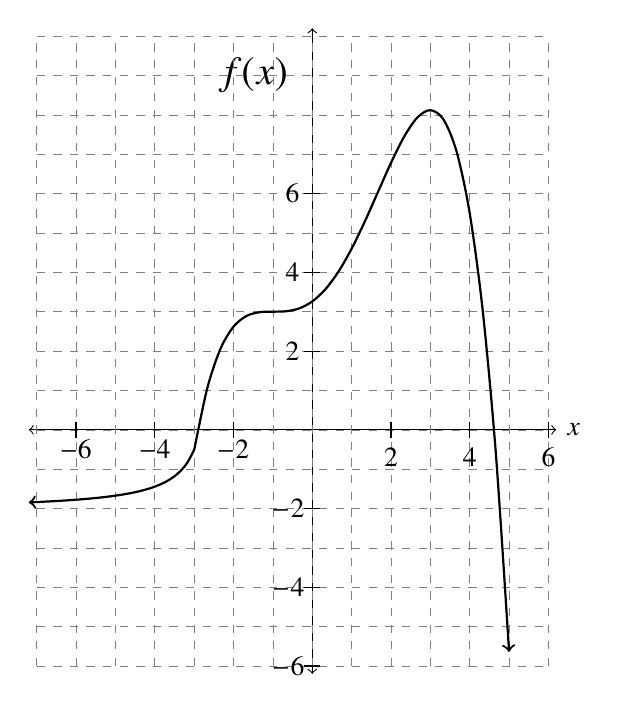
\begin{tikzpicture}[scale=0.5]
\node at (-1.5,9){\Large{$f(x)$}};
\draw[<->] (-7.2,0) -- (6.2,0) node[right] {$x$};
\draw[<->] (0,-6.2) -- (0,10.2); 
\draw[help lines, dashed] (-7,-6) grid (6,10);
\draw[domain=-3:5, smooth, variable=\x,->,thick] plot ({\x},{3-0.02*(\x+1)*(\x+1)*(\x+1)*(3*\x-13)});
\draw[domain=-7.2:-3, smooth, variable=\x,< -,thick] plot ({\x},{-1/(\x+2.35)-2.05});
\foreach \i in {2,4,6}{
	\node at (\i,-.7){$\i$};
	\draw (\i,0.2) -- (\i, -.2);
	\draw (-\i,0.2) -- (-\i, -.2);
	\draw (0.2,\i) -- (-.2,\i);
	\draw (0.2,-\i) -- (-.2,-\i);
	\node at (-\i,-.5){$-\i$};
	\node at (-.5,\i){$\i$};
	\node at (-.6,-\i){$-\i$};
	}
\end{tikzpicture}
\end{center}

\begin{enumerate}
\item List the $x$-values of all critical  numbers of $f.$\\

\vfill

\item Use the graph of $f(x)$ to sketch the graph of $f'(x)$ on the set of axes below.\\
\begin{center}
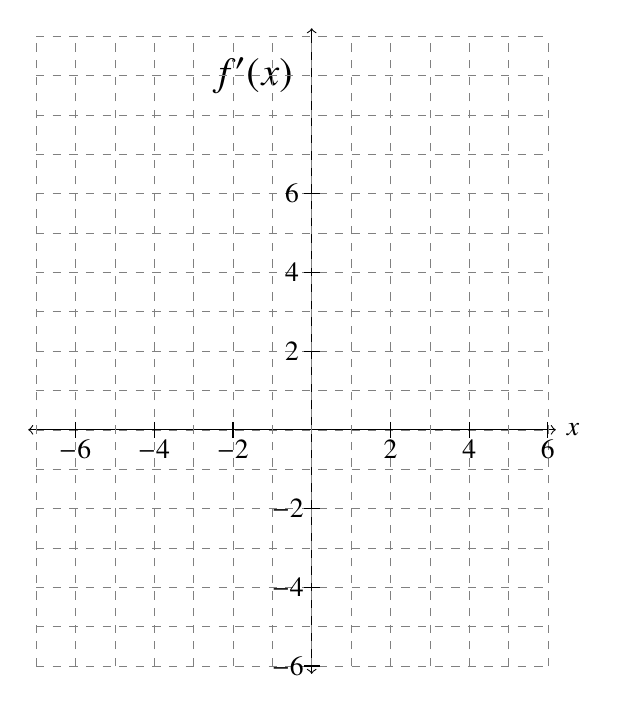
\begin{tikzpicture}[scale=0.5]
\node at (-1.5,9){\Large{$f'(x)$}};
\draw[<->] (-7.2,0) -- (6.2,0) node[right] {$x$};
\draw[<->] (0,-6.2) -- (0,10.2); 
\draw[help lines, dashed] (-7,-6) grid (6,10);
\foreach \i in {2,4,6}{
	\node at (\i,-.5){$\i$};
	\node at (-\i,-.5){$-\i$};
	\node at (-.5,\i){$\i$};
	\node at (-.6,-\i){$-\i$};
	\draw (\i,0.2) -- (\i, -.2);
	\draw (-\i,0.2) -- (-\i, -.2);
	\draw (0.2,\i) -- (-.2,\i);
	\draw (0.2,-\i) -- (-.2,-\i);
	}
\end{tikzpicture}
\end{center}
 \end{enumerate}
\newpage

\problem{10 points} The function $A(x)$ is graphed below. 

\begin{center}
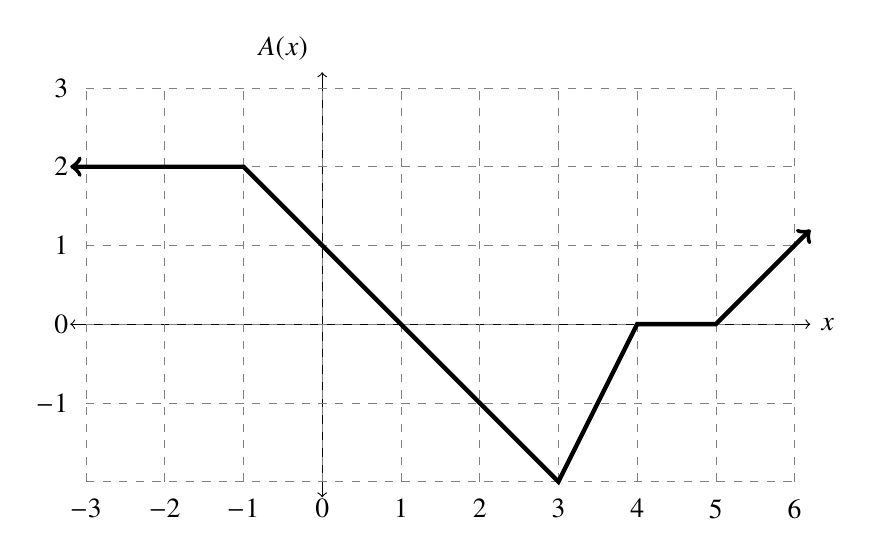
\begin{tikzpicture}[scale=1]
\draw[<->] (-3.2,0) -- (6.2,0) node[right] {$x$};
\draw[<->] (0,-2.2) -- (0,3.2); %node[left] {$A(x)$};
\draw (-.5, 3.5) node{$A(x)$};
\draw[help lines, dashed] (-3,-2) grid (6,3);
\draw[style= ultra thick,<->] (-3.2,2) --  (-1,2)--(1,0) -- (3,-2)--(4,0)--(5,0)--(6.2,1.2);
\foreach \x in {-3,-2,-1,0,1,2,3,4,5,6}
\draw (\x,-2.1) node[below] {$\x$};
\foreach \y in {-1,0,1,2,3}
\draw (-3.1,\y) node[left] {$\y$};
%\node[fill=white, minimum size=1pt,circle,draw,scale=.55] at (-2,2){};
%\node[fill=black, minimum size=1pt,circle,draw,scale=.5] at (-2,1){};
\end{tikzpicture}
\end{center}

\bigskip
\subproblem{}  $A(0)=$\\

\subproblem{}  $A'(0)=$\\

\subproblem{} At what $x$ values, if any, does $A'(x)$ not exist?
\vfill

\subproblem{} By using your knowledge of areas, evaluate $\displaystyle \int_{-2}^{4} A(x)\,dx$.

\vfill
For parts (e)-(g), let  $H(x) =\displaystyle \int_0^x A(s)\,ds$.

\subproblem{} What is the value of $H(2)$?

\vfill

\subproblem{} What is the value of $H'(2)$?

\vfill

\subproblem{} Where on the interval $[0,6]$ is $H(x)$ decreasing? 
\vfill
 

\newpage
\problem{10 points} The height of a right circular cylinder is increasing at rate of 3 meters per second while its volume remains constant.  (See figure below.) At what rate is the radius  changing when the radius and height are both 10 meters? \\

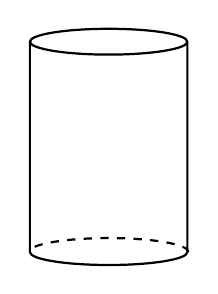
\begin{tikzpicture}
\node[cylinder, thick, aspect=1.4,shape border rotate=120, draw,minimum height=3cm,minimum width=2cm] (A)
{};
\draw[dashed, thick]
    let \p1 = ($ (A.after bottom) - (A.before bottom) $),
        \n1 = {0.5*veclen(\x1,\y1)},
        \p2 = ($ (A.bottom) - (A.after bottom)!.5!(A.before bottom) $),
        \n2 = {veclen(\x2,\y2)}
  in
    (A.before bottom) arc [start angle=0, end angle=180,
    x radius=\n1, y radius=\n2];
\end{tikzpicture}
\newpage
\problem{10 points}  Find any horizontal or vertical asymptotes for the function $f(x)=\frac{2x^2-3x}{5x^2-10}.$ Use limits to justify your answer(s). If no asymptote exists, explain why.\\
\vfill


\problem{10 points} A homeowner wants to minimize the cost of heating a building over the next 10 years. Adding $x$ inches of insulation in the attic costs \$100 per inch and results in heating costs of $1000/(2+x)$ dollars over 1 year. How many inches of insulation should be installed in order the minimize the total costs over a 10 year period? Justify your answer. (By \emph{total costs}, we mean both the initial cost of insulating the building plus the annual heating costs.)
\vfill
\newpage
\problem{10 points} Evaluate the integrals below. Note that these problems will be graded \emph{largely} by the quality of the work written. So make sure to include proper notation and compete steps.\\

\subproblem{} $\displaystyle{\int \sin(2 x)+\frac{(1+\ln x )^2}{x} dx}$
\vfill

\subproblem{} $\displaystyle{\int_0^2 (1+xe^{\pi x^2}) dx}$
\vfill

\newpage
\problem{10 points} Use $f$, $f'$ and $f''$ to answer the questions below.

$$f(x)=x \sqrt[3]{x^2-5} \quad \quad f'(x)=\frac{5(x^2-3)}{3(x^2-5)^{2/3}} \quad \quad f''(x)=\frac{10x(x^2-9)}{9(x^2-5)^{5/3}}.$$

\subproblem{} Determine all critical numbers of the function $f.$ Show how you obtain your answer.\\
\vspace{2in}
\subproblem{} For each critical number of $f$, classify it as a local minimum, a local maximum or neither. Show how you obtain your answer.\\
\vfill


\newpage
\problem{10 points} Short Answer
\subproblem{} A population of chickadees is increasing at a rate of $r(t)$ chickadees per year. What does $\displaystyle{\int_1^4 r(t) \: dt=400}$ mean? Make sure to include units in your answer.
\vfill
\subproblem{} Let $y=-3+5(x-4)$ be an equation of the tangent line to the graph of $f(x)$ at $x=4.$ Is it possible to determine $f(4)$ or $f'(4)$? Explain your answer.
\vfill
\subproblem{} Let $C(T)$ be the number of chirps per second of a male cricket as a function of temperature, $T$, in degrees Fahrenheit. In the context of the problem, interpret $C'(70)=2.$ Make sure to include units in your answer.
\vfill

\newpage

\problem{10 points} The acceleration function (in $m/s^2$), the initial velocity, and the initial position are given for a particle moving along a line. Find an expression for position, $s$, at time $t.$\\

$$ a(t)=\frac{12}{(1+t)^3}, \quad v(0)=0, \quad s(0)=0$$






 
 
 
 

\end{document}
%%%%%%%%%%%%%%%%%%%%%%%%%%
%%%%%%%END
%%%%%%%%%%%%%%%%%%%%%%%%%%


 